\section{Proposed approach}

Given a collection of existing DSLs (that we term as the \textit{input set}) our approach is intended to identify commonalities --and so, potential reuse--. Then, we evaluate those commonalities in order to know if the input set is a good candidates to a reverse engineering method that permits to exploit the existing potential reuse. The reminder of this section explain how we tackle this problem.

\subsection{Identifying commonalities}
\label{sec:metrics}

We start by identifying commonalities among the DSLs in the input set. In other words, we start by identifying intersections among DSL specifications (see Figure \ref{fig:domains}). To this end, we need to take into account thee considerations.

\vspace{-2mm}
\subsubsection{Consideration 1:} Commonalities can appear not only at the level of the syntax but also at the level of the semantics. Hence, the analysis should be performed in both, metamodels and domain-specific actions.

Our solution to this first consideration relies in two functions. The first one ($I_{syn}$), receives a set of metamodels and returns the set of metaclasses that are contained in all the input metamodels. 

\begin{equation}
  I_{syn} : set(MM) \rightarrow set(MC)
\end{equation}
\vspace{-2mm}
\begin{equation}
  I_{syn}(mms) = \bigcap _{i=0}^{|mms|}mms_i
\end{equation}

The second function ($I_{sem}$) does the proper for the case of the aspects. That is, it receives a set of aspects and returns the set of domain specific actions that are contained in all the input aspects. The implementation of these functions is based on static analysis of metamodels and aspects.

\begin{equation}
  I_{sem} : set(A) \rightarrow set(DSA)
\end{equation}
\vspace{-2mm}
\begin{equation}
  I_{sem}(dsas) = \bigcap _{i=0}^{|dsas|}dsas_i
\end{equation}

\vspace{-2mm}
\subsubsection{Consideration 2:} So far, we have defined a syntactic intersection as a set of metaclasses that are equal in two or more DSLs. Similarly, we define semantic intersection as a set of domain-specific actions that are equal in two or more DSLs. However, at this point we need to clearly define the notion of equality between metaclasses and domain-specific actions. That is, we need to establish the criteria under we consider that two metaclasses/domain-specific actions are equal.

\begin{itemize}
\item \textbf{Comparison of metaclasses:} The name of a metaclass usually corresponds to a word that evokes the domain concept the metaclass represents. Thus, intuitively one can think that a first approach to compare meta-classes is by comparing their names. As we will see later in this paper, this approach results quite useful and it is quite probable that, we can find potential reuse.

\begin{equation}
  \doteq~: MC \times MC \rightarrow bool
\end{equation}
\vspace{-1mm}
\begin{equation}
\begin{split}
  MC_{A} \doteq MC_{B} &= true \implies \\
   & MC_{A}.name = MC_{B}.name
 \end{split}
\end{equation}

\vspace{2mm}
\hspace{3mm} Unfortunately, comparison of metaclasses by using only their names might have some problems. There are cases in which two meta-classes with the same name are not exactly the same since they do not represent the same domain concept or because there are domains that use similar vocabulary. In such cases, an approach that certainly helps is to compare meta-classes not only by their names but also by their attributes and references. Hence, we define a second comparison operator for metaclasses i.e., $\doteqdot $.

\begin{equation}
  \doteqdot~: MC \times MC \rightarrow bool
\end{equation}
\vspace{-1mm}
\begin{equation}
\begin{split}
  MC_{A} \doteqdot MC_{B} &= true \implies \\
   & MC_{A}.name = MC_{B}.name ~ \wedge \\
   & \forall a_1 \in MC_{A}.attr \mid (\exists a_2 \in MC_{B}.attr \mid a_1 = a_2) ~ \wedge \\
   & \forall r_1 \in MC_{A}.refs \mid (\exists r_2 \in MC_{B}.refs \mid r_1 = r_2)
  \end{split}
\end{equation}



\vspace{2mm}
\hspace{3mm} Although this second approach might be too restrictive, it implies that the specification of the two meta-classes are exactly the same so potential reuse is guaranteed. At the implementation we provide support for the two comparison approaches explained above. However, additional comparison operators such as the surveyed in \cite{Lafi:2011} can be easily incorporated.

\vspace{2mm}

\item \textbf{Comparing domain-specific actions:} Like methods in Java, domain-specific actions have a signature that specifies its contract (i.e., return type, visibility, parameters, name, and so on), and a body where the behavior is actually implemented. In that sense, the comparison of two domain-specific actions can be performed by checking if their signatures are equal. This approach is practical and also reflects potential reuse; one might think that the probability that two domain-specific actions with the same signatures are the same is elevated.

\begin{equation}
  \circeq~: DSA \times DSA \rightarrow bool
\end{equation}
\vspace{-1mm}
\begin{equation}
\begin{split}
  DSA_{A} & \circeq DSA_{B} = true \implies \\
   & DSA_{A}.name = DSA_{B}.name ~ \wedge \\
   & DSA_{A}.returnType = DSA_{B}.returnType ~ \wedge \\
   & DSA_{A}.visibility = DSA_{B}.visibility ~ \wedge \\
   & \forall p_1 \in DSA_{A}.params \mid (\exists p_2 \in DSA_{B}.params \mid p_1 = p_2)
 \end{split}
\end{equation}

\vspace{2mm}
\hspace{3mm} However, as the reader might imagine, there are cases in which signatures comparison is not enough. Two domain-specific actions defined in different DSLs can perform different computations even if they have the same signatures. As a result, a second approach relies in the comparison of the bodies of the domain-specific actions. Note that such comparison can be arbitrary complex task. Indeed, if we try to compare  the behavior of the actions we will have to deal with the semantic equivalence problem that, indeed, is known as be undecidable \cite{Lucanu:2013}. In this case, we a conservative approach is to compare only the structure (abstract syntax tree) body of the domain-specific action. In our approach we support both comparison operators: the one based on the signature and the one based on the signature and the body. To the later, we use the API for java code comparison proposed in \cite{Biegel:2010}. 

\begin{equation}
  \triangleq~: DSA \times DSA \rightarrow bool
\end{equation}
\vspace{-1mm}
\begin{equation}
\begin{split}
  DSA_{A} \triangleq DSA_{B} & = true \implies \\
   & DSA_{A} \circeq DSA_{B} ~ \wedge \\
   & DSA_{A}.AST = DSA_{B}.AST
 \end{split}
\end{equation}

\end{itemize}

\vspace{-2mm}
\subsubsection{Consideration 3:} Commonalities can be found between two ore more DSLs of the input set. That is, we can find metaclasses and domain specific actions that are shared by more than two DSLs. Hence, intersections should be searched among all the possible combinations of the DSLs in the input set. Once those functions are defined and implemented, the second phase is to use them in order to find the intersections among the DSLs of the input set. 


%It is worth nothing that there is this phenomenon of \textit{semantical variability}. A necessary condition to decide whether two language constructs are equivalent is that both, the metaclass and the associated domain-specific actions are equivalent. This condition guarantees that the specification is the same not only at the level of the abstract syntax but also at the level of the semantics. However, there is a phenomenon in the literature that corresponds to semantical variability \cite{Cengarle:2009}. There is semantical variability when there there are two constructs that have the same abstract syntax (i.e., their metaclasses are equal) but that differ in the domain-specific actions. This case is of interest for us because even in the presence of semantical variability we can have some potential reuse. If the metaclasses of two constructs are the same we can reuse them even if their domain-specific actions are different. 

\vspace{-2mm}
\subsubsection{Visualizing intersections:} After being tacckled the considerations mentioned below. We provide a graphical mechanism based on Venn Diagrams to visualize the results. The idea is that language designers can see intersections easily as the form of overlappings existing among the given set of DSLs.

Figure \ref{fig:shape} shows the Venn Diagram for the case of our motivating scenario. In that figure we can see that the family is an overlapping family in terms of the abstract syntax. In the case of the semantics the results are quite interesting. Note that depending on the type of comparison operator we have different results. When the comparison operator is the naming, we have the same overlapping shape that in the case of the abstract syntax. However, when the operators become more restrictive the overlapping region is reduced. 

\begin{figure}
\centering
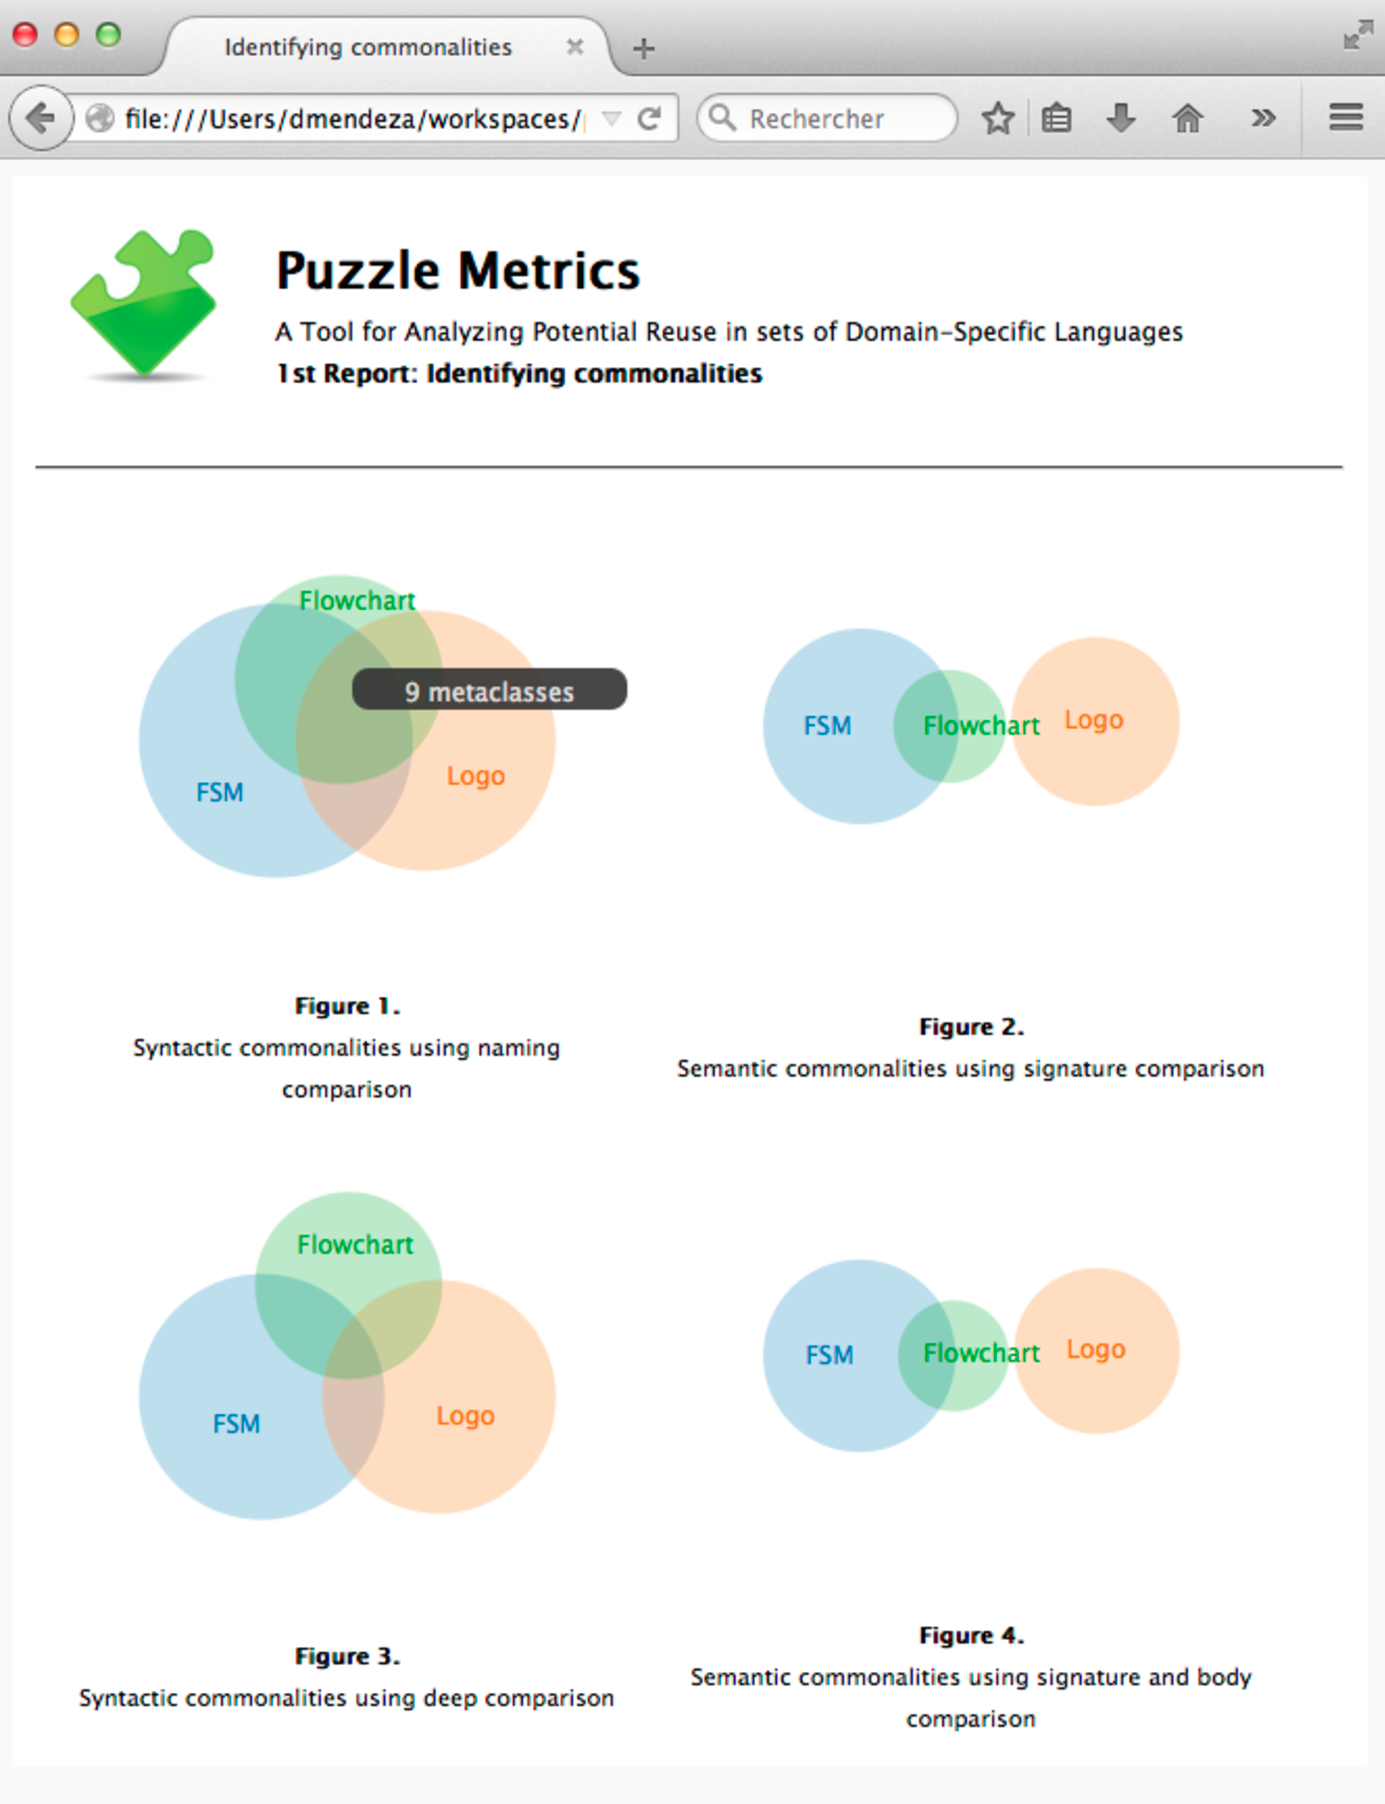
\includegraphics[width=1\linewidth]{images/domains-inaction.pdf}
\caption{Visualizing family's shape according to the selected comparison operator}
\label{fig:shape}
\end{figure}

%\vspace{-2mm}
%\subsubsection{Visualizing semantical variability:} Note that the phenomenon of semantical variability is evident in the example presented. Where there are syntactic commonalities between DSLs Logo and FSM, there are not semantic commonalities. As an additional feature of our approach, we provide a visualization of the semantical variability phenomenon. The idea is that language designers can see what are the variations in the domain specific actions.

\subsection{Objectively evaluating the potential reuse}

The second part of our analysis corresponds to a quantitative evaluation of potential reuse. To do so, we include the reuse metrics presented in X and we adapt them for the case of families of DSLs. In this section we present these metrics in terms of the formulas we used to compute them based on the basic definitions presented in section X. Besides, we show the output that our tool provides for our motivating scenario. It is important to remember that the computation of those metrics also depend on the comparison operator choosed for each case. 

\begin{itemize}
\item \textbf{Size of Commonality (SoC):} This metric shows the size of the core with respect to the rest of the family. It is calculated as the percentage of constructs/methods that are included in the core with respect to the union of the constructs/methods of all the DSLs of the family. 

\hspace{3mm} On the other hand, the larger the core the smaller the variability. So the amount of required decomposition is reduced and the variability model is simpler. So, one may think that a family where the core is big is a family where the variability is easier to manage. 

\vspace{2mm}
\item \textbf{Product-Related Reusability ($PRR_i$):}
This metric shows the percentage of reuse of each DSL with respect the core. Concretely, it shows for each product the amount of constructs/methods that are included in the core.

\hspace{3mm} This metric is important because we can detect the product more related to the core. This identification will be helpful at the moment of defining that core. 

\vspace{2mm}
\item \textbf{Individualization Ratio ($IR_i$):}
This metric shows the percentage of reuse of each DSL with respect the rest of the family. Concretely, it shows for each product the amount of constructs/methods that are included in at least another DSL that is member of the family.

\hspace{3mm} This metric is important because it allows the identification of the most isolated product as well as the most integrated to the family.

\vspace{2mm}
\item \textbf{Pairwise Relationship Ratio ($PWRR_{(i,j)}$):} 
This metric shows the percentage of reuse of each DSL with respect the each of the other DSLs that are members of the family. Concretely, it shows, for each product, the amount of constructs/methods that are included each of the other members of the family.
\end{itemize}

\subsubsection{Tool support.} Figure x shows the output of our tool. In this case, it receives a set of DSLs and it computes all the metrics explained above. 
